\documentclass{article} % For LaTeX2e
\usepackage{nips15submit_e,times}
\usepackage{hyperref}
\usepackage{url}
\usepackage{graphicx}
%\documentstyle[nips14submit_09,times,art10]{article} % For LaTeX 2.09


\title{Machine Learning Project}


\author{
Alex Brinkman\\
Robotics Institute\\
Carnegie Mellon University\\
Pittsburgh, PA 15213 \\
\texttt{abrinkma@andrew.cmu.edu} \\
\And
Abhishek Bhatia \\
Robotics Institute \\
Carnegie Mellon University\\
Pittsburgh, PA 15213 \\
\texttt{abhatia1@andrew.cmu.edu} \\
}

% The \author macro works with any number of authors. There are two commands
% used to separate the names and addresses of multiple authors: \And and \AND.
%
% Using \And between authors leaves it to \LaTeX{} to determine where to break
% the lines. Using \AND forces a linebreak at that point. So, if \LaTeX{}
% puts 3 of 4 authors names on the first line, and the last on the second
% line, try using \AND instead of \And before the third author name.

\newcommand{\fix}{\marginpar{FIX}}
\newcommand{\new}{\marginpar{NEW}}

\nipsfinalcopy % Uncomment for camera-ready version

\begin{document}


\maketitle

\begin{abstract}
abstract goes here
\end{abstract}

\section{Part 1}

The goal of the project for part 1 is to classify subject behavior baed on raw voxel activation values.  The final approach developed to achieve this goal includes an SVM classifier, custom feature extraction, and a voting method. The resulting accuracy was 60.47\% on the holdout data set.
\subsection{SVM Classifier}
Abhishek
\subsection{Custom Feature Extraction}

The custom feature extraction....

\begin{figure}[h]
\begin{center}
%\framebox[4.0in]{$\;$}
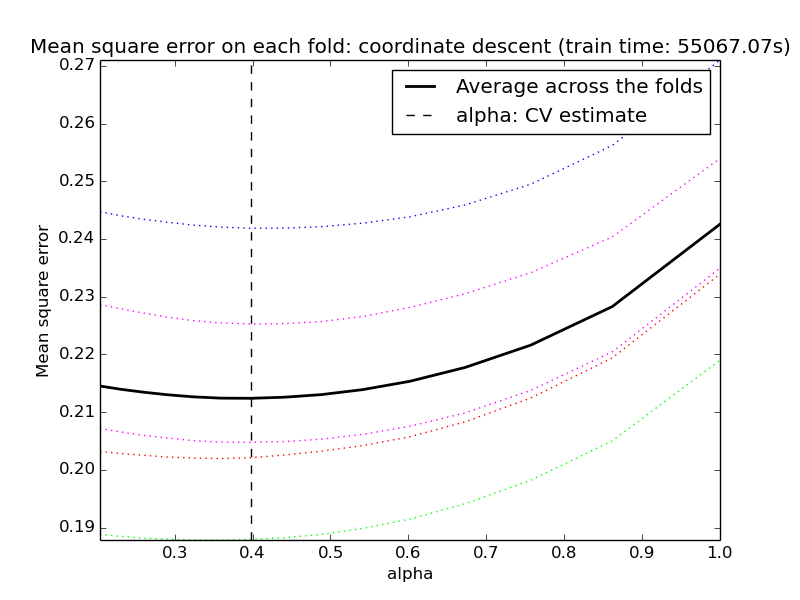
\includegraphics[scale=.5]{media/cross_validation_figure_2.png}
\end{center}
\caption{Sample figure caption.}
\end{figure}

\begin{table}[t]
\caption{Sample table title}
\label{sample-table}
\begin{center}
\begin{tabular}{ll}
\multicolumn{1}{c}{\bf HEADING C1}  &\multicolumn{1}{c}{\bf HEADING C2}
\\ \hline \\
r1c1   &r1c2       \\
r2c1   &r2c2 \\
etc		&etc\\
\end{tabular}
\end{center}
\end{table}

\subsection{Voting Method}

\section{Part 2}
\subsection{Ridge and Lasso Classifiers}
\subsection{MultiTaskLasso Cross Validation}
\subsection{Euclidean Clustering}


\section{Part 3}

\subsection{Hypothesis}

\subsection{Experiment}

\subsection{Results}




\subsubsection*{References}

\small{
[1] Scikit-learn: Machine Learning in Python, Pedregosa et al., JMLR 12, pp. 2825-2830, 2011.
}

\end{document}
